\chapter{Funciones elementales}

\section{Funciones multivaluadas} \label{Multivaluadas}

\subsection{Definiciones}

En cursos anteriores hemos aprendido que una función es una aplicación que a cada elemento del dominio le hace corresponder un único elemento del codominio. En variable compleja también ocurre lo mismo, sin embargo, es conveniente trabajar con aplicaciones que a cada número complejo le asocia un conjunto de números complejos.

\begin{defi}
Sea la función compleja $w = f(z)$, si para cada valor de la variable independiente $z$ existe uno y solo un punto imagen $w$, se dice que la función es \textbf{uniforme} o \textbf{monovaluada} o \textbf{univaluada}. En caso contrario, la función se dice \textbf{multiforme} o \textbf{multivaluada}.
\end{defi}

Por definición, una función es \textbf{multivaluada} si para cada valor de la variable $z$ existen más de un valor de la variable $w$. Los ejemplos más notables que hemos visto hasta ahora son: $arg(z)$ y $z^{1/n}$. La mayoría de las funciones multivaluadas aparecen cuando se intenta determinar la inversa de funciones univaluadas no inyectivas.

\begin{figure}[H]
    \centering
    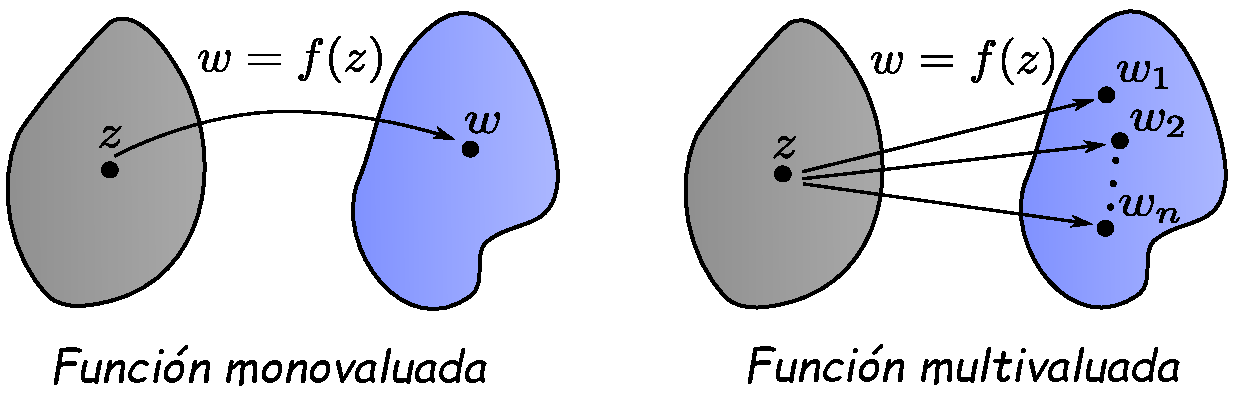
\includegraphics[scale=0.6]{Figuras/Funciones_Multivaluadas.pdf}
    \caption{Función multivaluada.}
    \label{MultiF}
\end{figure}

Para funciones multivaluadas, nos interesará conocer el mayor dominio en donde ésta sea una función monovaluada.

\begin{defi}
Sea $f(z)$ una función multivaluada definida en un dominio $D \subseteq \mathbb{C}$. Diremos que $F(z)$ es una \textbf{rama} o \textbf{determinación continua} de $f(z)$ en $D$ si:
\begin{enumerate}
    \item $F(z)$ es una función monovaluada.
    
    \item $F(z)$ es uno de los posibles valores de $f(z)$ para cada $z \in D$.
    
    \item $F$ es continua en $D$.
\end{enumerate}
\end{defi}

\begin{ejemplo}
Recordemos que si se restringe el argumento de un complejo a $- \pi < \theta \leq \pi$, obtenemos el argumento principal $Arg(z)$. La función $f(z) = Arg(z)$ es monovaluada y continua en $\mathbb{C} \setminus \,]- \infty,0]$ y en el semieje real negativo presenta una discontinuidad de salto. En otras palabras,  $Arg(z)$ es una \textit{rama} de la función multivaluada $arg(z)$ en $\mathbb{C} \setminus \,]- \infty,0]$.
\end{ejemplo}

\begin{ejemplo}
Sabemos que la raíces cúbicas de un número complejo $z = r e^{i \theta}$ están dadas por 
$$\sqrt[3]{r} \exp \left( i \frac{\theta + 2k\pi}{3} \right), \quad k = 0,1,2.$$

Por lo tanto, para cada $k$ se obtienen las tres ramas de la función $w = f(z) = z^{1/3}$:
\begin{align*}
w_1 &= |z|^{1/3} e^{i\theta/3}  \\
w_2 &= |z|^{1/3} e^{i(\theta/3 + 2\pi/3)}  \\
w_3 &= |z|^{1/3} e^{i(\theta/3 + 4\pi/3)}    
\end{align*}

donde $0 < \theta < 2\pi$. 

Notemos que los $z \in \mathbb{C}$ tales que $\theta = 0, 2\pi$ se omiten, pues la rama dejaría de ser continua.
\end{ejemplo}

\subsection{Ramas y puntos de ramificación}

En esta subsección profundizaremos el concepto de rama de una función multivaluada, para ello comencemos con un ejemplo.

\begin{ejemplo} \label{EjemploRaiz}
Consideremos la función $w = f(z) = \sqrt{z}$. Si $z = r e^{i\theta}$ las raíces cuadradas están dadas por
$$\sqrt{r} \exp \left(\frac{\theta + 2k\pi}{2} \right), \quad k = 0,1.$$

Entonces, para cada $k$ se obtienen las dos ramas de la función:
\begin{align*}
    w_1 &= \sqrt{r} e^{i \theta/2}, \\
    w_2 &= \sqrt{r} e^{i (\theta/2 + \pi)} = -w_1.
\end{align*}

Para $\theta \in ]0, 2\pi[$, grafiquemos las ramas de la función, ver figura \ref{fig:Raiz1}. Notemos que omitimos los extremos $\theta = 0,2\pi$ y el origen, es decir, el conjunto
\begin{equation}
\{ z \in \mathbb{C} : Re(z) \geq 0 \wedge Im(z) = 0\},    \label{CorteRama1}
\end{equation}

porque la rama dejaría de ser continua. Observemos que la curva que separa ambas ramas es el eje real, la cual correspondería al evaluar $f$ en \eqref{CorteRama1}. Debido a ésto este conjunto es conocido como \textit{corte de ramificación}.

\begin{figure}[H]
    \centering
    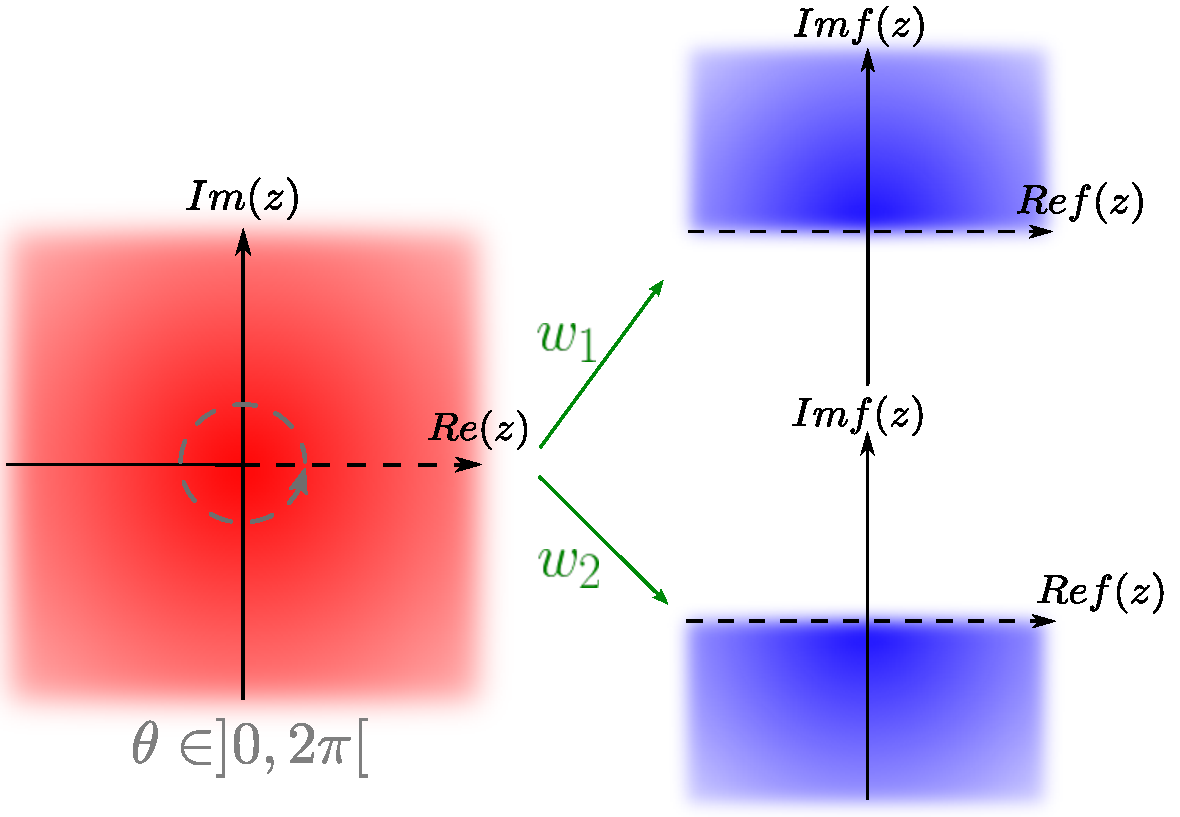
\includegraphics[scale = 0.5]{Figuras/RaizCuadrada1.pdf}
    \caption{Gráficas de las ramas de la función raíz cuadrada $f(z) = \sqrt{z}$ para $z = r e^{i\theta}$ con $\theta \in ]0,2\pi[$.}
    \label{fig:Raiz1}
\end{figure}

¿Qué pasaría si consideramos otro intervalo de longitud $2\pi$ como $]-\pi, \pi[$?
\\

Para $\theta \in ]-\pi, \pi[$, las gráficas de las ramas de la función están representadas en la figura \ref{fig:Raiz2}. En este caso, el corte de ramificación corresponde al conjunto 
\begin{equation}
\{ z \in \mathbb{C} : Re(z) \leq 0 \wedge Im(z) = 0\},    \label{CorteRama2}
\end{equation}

\begin{figure}[H]
    \centering
    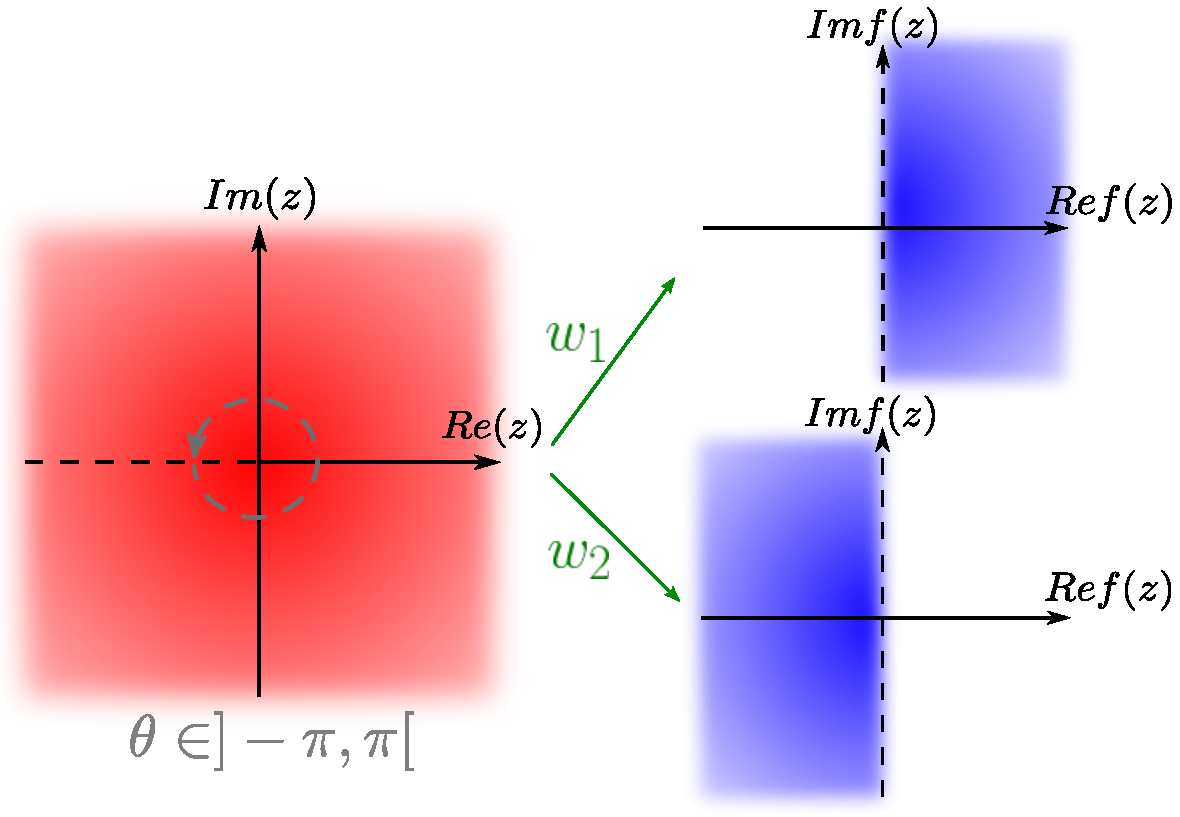
\includegraphics[scale = 0.5]{Figuras/RaizCuadrada2.pdf}
    \caption{Gráficas de las ramas de la función raíz cuadrada $f(z) = \sqrt{z}$ para $z = r e^{i\theta}$ con $\theta \in ]-\pi,\pi[$.}
    \label{fig:Raiz2}
\end{figure}

\end{ejemplo}

\begin{defi}
Un \textbf{corte de ramificación} es una línea (habitualmente recta) que separa dos ramas de una misma función multivaluada. Equivalentemente, es la línea en la que una rama se hace discontinua.
\end{defi}

\begin{defi}
Sea $f(z)$ una función multivaluada y $z_0$ un punto de su dominio. Decimos que $z_0$ es un \textbf{punto de ramificación} de $f(z)$ si una vuelta alrededor de $z_0$ (y suficientemente cerca a $z_0$) produce un cambio de rama de la función. 
\end{defi}

\begin{ejemplo}
El complejo $z = 0$ es un punto de ramificación de $f(z) = \sqrt{z}$.
\end{ejemplo}

\textbf{Observación:} Los cortes de ramificación son curvas por las que hacemos discontinuas las ramas y que impiden que podamos dar una vuelta completa alrededor de un punto de ramificación. Como pudimos notar en el ejemplo \ref{EjemploRaiz}, los cortes de ramificación no son únicos y podemos elegirlos según nos convenga.

Así cada punto de ramificación deben tener en común todos los cortes de $f$.

\section{Función exponencial}

\begin{defi}
Llamaremos \textbf{función exponencial} a $f: \mathbb{C} \longrightarrow \mathbb{C}$ tal que
$$f(z) = e^x(\cos y + i \sin y),$$

la cual denotamos por $e^z = \exp(z)$.
\end{defi}

\begin{propo}
\ 

\begin{enumerate}
    \item La función exponencial $f(z) = e^z$ es entera y $f'(z) = f(z)$.
    
    \item La función exponencial es la única función que cumple $f'(z) = f(z)$ con $f$ entera y $f(x + i0) = e^x$ (se recupera la exponencial real).
\end{enumerate}
\end{propo}

\begin{proof}
\ 

\begin{enumerate}
    \item Las funciones componentes de $e^z$ son
$$u(x,y) = e^x \cos y; \quad v(x,y) = e^x \sin y.$$

Además, 
\begin{align*}
u_x &= e^x \cos y = v_y, \\
u_y &= -e^x \sin y = -v_x,
\end{align*}

es decir, $f$ es una función \underline{entera} y 
\begin{equation*}
f'(z) = f(z) ~~\mbox{o}~~ \frac{d}{dz}(e^z) = \frac{d}{dz}(\exp(z)) = e^z.
\end{equation*}

\item Supongamos que la función $f(z) = u(x,y) + i v(x,y)$ es una función entera con $f'(z) = f(z)$, luego ésta satisface las ecuaciones de Cauchy-Riemann y 
$$f'(z) = u_x(x,y) + i v_x(x,y) = u(x,y) + iv(x,y) ~\Rightarrow~ \left\{ \begin{array}{ccc}
u_x(x,y) &=& u(x,y) \\
v_x(x,y) &=& v(x,y) 
\end{array} \right. .$$

De la primera ecuación, tenemos que
\begin{align*}
u_x (x,y) - u(x,y) = 0 \quad \color{red}{/\cdot e^{-x}} &\Rightarrow e^{-x} u_x (x,y) - e^{-x} u(x,y) = 0 \\
&\Rightarrow \frac{\partial}{\partial x} \left[ u(x,y)e^{-x} \right] = 0 \\
&\Rightarrow  u(x,y)e^{-x} = \phi(y) \\
&\Rightarrow  u(x,y) = e^{x} \phi(y).
\end{align*}

Análogamente se prueba que 
$$v(x,y) = e^x \psi(y).$$

Ahora, que $f$ sea entera nos dice también que sus componentes son funciones armónicas, en particular se cumple 
\begin{equation*}
u_{xx}(x,y) + u_{yy}(x,y) = 0 ~\Rightarrow~ e^x \phi(y) + e^x \phi''(y) = 0 ~\Rightarrow ~\phi''(y) + \phi(y) = 0.
\end{equation*} 

La EDO de segundo orden homogénea tiene como solución
$$\phi(y) = A \sin y + B \cos y,$$

con $A$ y $B$ constantes de integración.

Ahora, si hacemos lo mismo para $\psi(y)$ obtendríamos otras constantes de integración que a priori no tienen porqué ser iguales a las de $\phi$, sin embargo, de la ecuación de Cauchy-Riemann, $u_y = -v_x$ se tiene que
\begin{equation*}
e^x \phi'(y) = -e^x \psi(y) ~\Rightarrow~ \psi(y) = -A \cos y + B \sin y.
\end{equation*}

Si además añadimos la condición que  
$$f(x+i0) = u(x,0) + i v(x,0) = e^x,$$

obtenemos 
$$e^x (B - iA) = e^x ~\Rightarrow~ B = 1 + iA.$$

Entonces,
$$f(z) = u(x,y) + i v(x,y) = e^x ((B-iA) \cos y + (A + iB)\sin y) = e^x (\cos y + i \sin y).$$
\end{enumerate}
\end{proof}



La forma más compacta 
$$e^z = e^xe^{iy}$$

de la exponencial permite demostrar la siguiente proposición.

\begin{propo}[Propiedades de la exponencial]
Sean $z_1, z_2 \in \mathbb{C}$, se verifica: 

\begin{enumerate}
\item $\exp(z_1 + z_2) = \exp(z_1) \exp(z_2)$.

\item $\frac{\exp(z_1)}{\exp(z_2)} = \exp(z_1 - z_2)$.

\item $e^0= 1; ~ 1/e^z = e^{-z}; ~ (e^z)^n = e^{nz}, \quad n \in \mathbb{Z}.$
\end{enumerate}
\end{propo}

\begin{proof}
Sean $z_1 = x_1 + iy_1$, $z_2 = x_2 + iy_2$ números complejos cualesquiera. 

\begin{enumerate}
\item 
\begin{align*}
\exp(z_1 + z_2) = \exp((x_1+x_2) + i (y_1+y_2)) &= e^{x_1 + x_2} e^{i(y_1+y_2)} \\
&=  [e^{x_1}e^{x_2}][e^{iy_1} e^{iy_2}] \\
&= [e^{x_1} e^{iy_1}][e^{x_2} e^{iy_2}] \\
 &= \exp(z_1) \exp(z_2).
\end{align*}

\item 
\begin{align*}
\frac{\exp(z_1)}{\exp(z_2)} = \frac{\exp(x_1 + iy_1)}{\exp(x_2+iy_2)} &= \frac{e^{x_1} e^{iy_1}}{e^{x_2} e^{iy_2} } \\
&=  \left[\frac{e^{x_1}}{e^{x_2}}\right]\left[\frac{e^{iy_1}}{e^{iy_2}}\right] \\
&= e^{x_1-x_2} e^{i(y_1-y_2)} \\
&= \exp(z_1-z_2).
\end{align*}

\item Es fácil de ver que $e^0 = e^{0+i0} = 1$, luego 
$$\frac{1}{e^{z}} = \frac{e^0}{e^{z}} = e^{-z}.$$

Probemos por inducción que $(e^{z})^n = e^{nz}$, $n \in \mathbb{Z}$.

Para $n = 0,1$; $(e^{z})^0 = 1 = e^{0\cdot z}$ y $e^z = e^{1\cdot z}$. 

Suponiendo que para $n \in \mathbb{N}$ se verifica 
$$(e^{z})^n = e^{nz},$$

tenemos que 
$$(e^{z})^{n+1} = (e^{z})^n e^z = e^{nz} e^z = e^{(n+1)z}.$$

Por lo tanto, 
$$(e^{z})^n = e^{nz}; \quad n = 0,1,2, \dots$$

Ahora, haciendo $m = -n$ con $n \in \mathbb{N}$, resulta que 
$$(e^z)^m = (e^z)^{-n} = ((e^{z})^{-1})^n = \left(\frac{1}{e^z}\right)^n = (e^{-z})^n = e^{-nz} = e^{mz}. $$

Finalmente, hemos probado que 
$$(e^{z})^n = e^{nz}, \quad n \in \mathbb{Z}.$$

\end{enumerate}
\end{proof}

Veamos ahora más propiedades de la función exponencial

\newpage
\begin{propo}
\ 

\begin{enumerate}
    \item El recorrido de la función exponencial es $\mathbb{C} \setminus \{0\}$.
    
    \item $e^z$ no es inyectiva, es más, tiene periodo $2\pi i$.
\end{enumerate}
\end{propo}

\begin{proof}
\ 

\begin{enumerate}
    \item Escribamos $\exp(z)$ como 
$$e^z = \rho(\cos\phi + i \sin\phi)$$

donde $\rho = e^x$ y $\phi = y$. Así, 
$$|e^z| = e^x > 0; ~ arg(e^z) = y + 2n\pi, \quad n \in \mathbb{Z}.$$

Nótese que al ser $|e^z|$ siempre positivo, 
$$\forall z \in \mathbb{C}: ~w = e^z \neq 0.$$

Por otro lado, sea
$$w = r (\cos\theta + i \sin \theta), \quad r >0$$

un complejo distinto de cero. Se define el complejo 
$$z = \ln r + i\theta.$$

Calculemos 
$$e^z = e^{\ln r + i\theta} = e^{\ln r} e^{i\theta} = r (\cos \theta + i\sin\theta) = w.$$

Por lo tanto, todo punto $w$ en el plano complejo menos el origen, es imagen de un $z \in \mathbb{C}$, o sea,
$$Rec(e^z) = \mathbb{C} - \{0\}.$$

\item Ahora como 
\begin{align*}
\cos\theta &= \cos(\theta + 2\pi k ) \\
\sin\theta &= \sin(\theta + 2\pi k)
\end{align*}

con $k \in \mathbb{Z}$, se tiene que la función exponencial \underline{no es inyectiva}, más aún,
$$e^{z + 2\pi i} = e^z,$$

es decir, es \underline{periódica} de periodo $2\pi i$.
\end{enumerate}
\end{proof}

\textbf{Observación:} Si restringimos el dominio de $w = e^z$ a la franja
$$-\pi < Im(z) \leq \pi,$$

la función $w = e^z$ resulta ser inyectiva en esta franja.

Si 
$$w = r (\cos \Phi + i \sin\Phi),$$

donde $Arg(w) = \Phi$, entonces 
$$z = \ln r + i\Phi$$

es tal que 
$$e^{\ln r + i \Phi} = w.$$

\section{Funciones trigonométricas}

\begin{defi}
Llamaremos \textbf{funciones trigonométricas} a las siguientes funciones:
\begin{align*}
\sin z = \frac{e^{iz} - e^{-iz}}{2i} &\qquad \cos z = \frac{e^{iz} + e^{-iz}}{2} \\
\tan z = \frac{\sin z}{\cos z}; ~ \cos z\neq 0 &\qquad \cot z = \frac{\cos z}{\sin z};~\sin z \neq 0 \\
\sec z = \frac{1}{\cos z}; ~ \cos z \neq 0 &\qquad \csc z = \frac{1}{\sin z}; ~ \sin z \neq 0
\end{align*}
\end{defi}

\textbf{Observación:} Es directo de la definición que
$$e^{iz} = \cos z + i \sin z, \quad \forall z \in \mathbb{C}$$

y $\sin^2 z + \cos^2 z = 1$. En efecto,
\begin{align*}
    \sin^2 z + \cos^2 z  &= -\frac{(e^{iz} - e^{-iz})^2}{4} + \frac{(e^{iz} + e^{-iz})^2}{4} \\
    &= \frac{- e^{2iz} + 2 -  e^{-2iz} + e^{2iz} +2 +e^{-2iz}}{4} = 1.
\end{align*}

Determinemos sus derivadas:
\begin{align*}
\frac{d}{dz}[\sin z] &= \frac{1}{2i} [i e^{iz} + i e^{-iz}] = \frac{e^{iz} + e^{-iz}}{2} = \cos z, \\
\frac{d}{dz}[\cos z] &= \frac{1}{2} [i e^{iz} - i e^{-iz}] = - \frac{e^{iz} - e^{-iz}}{2i} = - \sin z, \\
\frac{d}{dz}[\tan z] &= \frac{\cos^2 z + \sin^2 z}{\cos^2 z} = \frac{1}{\cos^2 z} = \sec^2 z, \\
\frac{d}{dz} [\cot z] &= \frac{-\sin^2 z - \cos^2 z}{\sin^2 z} = -\frac{1}{\sin^2 z} = -\csc^2 z, \\
\frac{d}{dz}[\sec z] &= \frac{\sin z}{\cos^2 z} = \frac{1}{\cos z} \frac{\sin z}{\cos z}  = \sec z \tan z, \\
 \frac{d}{dz}[\csc z] &= - \frac{\cos z}{\sin^2 z} = -\frac{1}{\sin z} \frac{\cos z}{\sin z}  = -\csc z \cot z.
\end{align*}

Luego, podemos concluir que las funciones seno y coseno son enteras y las demás analíticas en su dominio de definición.

Note que las derivadas son las mismas que en el caso real, pero ¿conservarán más propiedades de las funciones trigonométricas reales?, por ejemplo, ¿la paridad?
\begin{align*}
\forall z \in \mathbb{C}:~ \sin(-z) &= \frac{e^{-iz} - e^{iz}}{2i} = - \frac{ e^{iz} - e^{-iz} }{2i} = - \sin z , \\
\cos(-z) &= \frac{e^{-iz} + e^{iz}}{2} =  \cos z.
\end{align*}

Entonces, la función seno compleja también es impar y la función coseno compleja es par. De la misma forma se puede probar que la tangente, la cotangente y la cosecante complejas son impares, y la secante compleja es par.

\begin{ejemplo}\label{PropiedadesTrigo}
Muestre que 

\begin{enumerate}
\item $\sin z = \sin x \cosh y + i \cos x \sinh y$.

\item $\cos z = \cos x \cosh y - i \sin x \sinh y$.

\item $\sin(iy) = i \sinh y$; $\cos(iy) = \cosh y$. 

\item $\sin(\overline{z}) = \overline{\sin z}$; $\cos(\overline{z}) = \overline{\cos z}$.
\end{enumerate}

\textbf{Solución:} Sea $z = x + iy \in \mathbb{C}$.

\begin{enumerate}
\item 
\begin{align*}
\sin z =\frac{e^{i(x+iy)} - e^{-i(x+iy)}}{2i} &= \frac{e^{-y + ix} - e^{y - ix}}{2i} \\
&= \frac{e^{-y} e^{ix} - e^{y} e^{-ix}}{2i} \\
&= \frac{e^{-y}(\cos x + i \sin x) - e^y (\cos x - i \sin x)}{2i} \qquad \mbox{(Identidad de Euler)}\\
&= \frac{\cos x (e^{-y} - e^y) + i \sin x (e^{-y} + e^y)}{2i} \cdot \frac{i}{i} \\
&= \sin x \frac{e^y + e^{-y}}{2} + i \cos x \frac{e^y-e^{-y}}{2} \\
&= \sin x \cosh y + i \cos x \sinh y.
\end{align*}

\item 
\begin{align*}
\cos z =\frac{e^{i(x+iy)} + e^{-i(x+iy)}}{2i} &= \frac{e^{-y + ix} + e^{y - ix}}{2} \\
&= \frac{e^{-y} e^{ix} + e^{y} e^{-ix}}{2} \\
&= \frac{e^{-y}(\cos x + i \sin x) + e^y (\cos x - i \sin x)}{2} \qquad \mbox{(Identidad de Euler)}\\
&= \cos x \frac{e^y + e^{-y}}{2} - i \sin x \frac{e^y-e^{-y}}{2} \\
&= \cos x \cosh y - i \sin x \sinh y.
\end{align*}

\item Usando lo demostrado en 1. y 2., tenemos que
\begin{align*}
\sin(iy) &= \sin(0) \cosh y + i \cos(0) \sinh y = i \sinh y, \\
\cos(iy) &= \cos(0) \cosh y - i \sin (0) \sinh y = \cosh y.
\end{align*}

\item Usando lo demostrado en 1., 2. y la paridad de las funciones hiperbólicas reales, tenemos que
\begin{align*}
\sin( \overline{z}) = \sin(x-iy) &= \sin x \cosh(-y) + i \cos x \sinh(-y) \\
&= \sin x \cosh(y) - i \cos x \sinh(y) \\
&= \overline{\sin x \cosh(y) + i \cos x \sinh(y)} \\
&= \overline{\sin z}, \\
\cos( \overline{z}) = \cos(x-iy) &= \cos x \cosh(-y) - i \sin x \sinh(-y) \\
&= \cos x \cosh(y) + i \sin x \sinh(y) \\
&= \overline{\cos x \cosh(y) - i \sin x \sinh(y)} \\
&= \overline{\cos z}.
\end{align*}
\end{enumerate}
\end{ejemplo}

\begin{ejemplo}
Muestre que las funciones trigonométricas son periódicas.
\\

\textbf{Solución:} Para todo $z = x+iy \in \mathbb{C}$, se tiene que 
\begin{align*}
\sin(z + 2\pi) &= \sin(x + 2\pi) \cosh y + i \cos(x + 2\pi) \sinh y = \sin x \cosh y + i \cos x \sinh y = \sin z. \\
\cos(z + 2\pi) &= \cos(x+2\pi) \cosh y - i \sin(x+2\pi) \sinh y = \cos x \cosh y - i \sin x \sinh y = \cos z
\end{align*}

Por lo tanto, la función seno y coseno son periódicas de periodo $2\pi$, de la misma forma se puede probar la misma periocidad para la secante y la cosecante. 

Con respecto a las funciones trigonométricas restantes, observemos que 
\begin{align*}
\tan(z + \pi) &= \frac{\sin(x + \pi) \cosh y + i \cos(x + \pi) \sinh y}{\cos(x+\pi) \cosh y - i \sin(x+\pi) \sinh y} = \frac{-(\sin x \cosh y + i \cos x \sinh y)}{-(\cos x\cosh y - i \sin x \sinh y)} = \tan z. \\
\cot(z + \pi) &= (\tan(z+\pi))^{-1} = (\tan z)^{-1} = \cot z,
\end{align*}

ésto es, la tangente y cotangente son periódicas de periodo $\pi$.

\end{ejemplo}

\begin{ejemplo}
Muestre que 
$$|\sin z|^2 = \sin^2 x + \sinh^2 y; ~ |\cos z|^2 = \cos^2x + \sinh^2y.$$

\textbf{Solución:} Usando lo demostrado en el ejemplo \ref{PropiedadesTrigo}, obtenemos que 
\begin{align*}
|\sin z|^2 &= \sin^2 x \cosh^2 y + \cos^2x \sinh^2 y  = \sin^2 x \cosh^2 y + \sinh^2 y - \sin^2 x \sinh^2 y =  \sin^2x + \sinh^2 y. \\
|\cos z|^2 &= \cos^2 x \cosh^2 y + \sin^2 x \sinh^2 y = \cos^2 x \cosh^2 y + \sinh^2 y - \cos^2 x \sinh^2 y = \cos^2 x + \sinh^2 y.
\end{align*}
\end{ejemplo}

\begin{ejemplo}
Encontrar las fórmulas para 
$$\sin(z_1 + z_2); ~ \cos(z_1+z_2); ~ \sin(2z);~ \cos(2z).$$

\textbf{Solución:} A partir de las propiedades de la exponencial, tenemos 
\begin{align*}
\sin(z_1 + z_2) &= \frac{e^{i(z_1 + z_2)} - e^{-i(z_1 + z_2)}}{2i} \\
&= \frac{e^{iz_1}e^{iz_2} - e^{-iz_1}e^{-iz_2} + e^{iz_1}e^{-iz_2} - e^{iz_1}e^{-iz_2} + e^{-iz_1}e^{iz_2} - e^{-iz_1}e^{iz_2} }{2i}  \\
&= \frac{(e^{iz_1} - e^{-iz_1})(e^{iz_2} + e^{-iz_2}) -e^{iz_1}e^{-iz_2} + e^{-iz_1}e^{iz_2}}{2i} \\
&= \frac{4i \sin z_1 \cos z_2 - (e^{i(z_1 - z_2)} - e^{-i(z_1 - z_2)}) }{2i} \\
&= 2\sin z_1 \cos z_2 - \sin(z_1 - z_2).
\end{align*}

Luego, 
\begin{align*}
2 \sin z_1 \cos z_2 = \sin(z_1 + z_2) + \sin(z_1 - z_2) ~\Rightarrow~ 2 \sin z_2 \cos z_1 &= \sin(z_2 + z_1) + \sin(z_2 - z_1) \\
&= \sin(z_1 + z_2) - \sin(z_1 - z_2).
\end{align*}

Sumando ambas expresiones:
$$\boxed{\sin(z_1 + z_2) = \sin z_1 \cos z_2 +\cos z_1 \sin z_2}$$ 

A partir de esta expresión es fácil de ver que
\begin{equation*}
\sin(2z) = 2 \sin z \cos z, \quad
\sin\left(z + \frac{\pi}{2} \right) = \cos z, \quad 
\cos\left( z + \frac{\pi}{2} \right) = - \sin z.
\end{equation*}

Entonces, 
\begin{align*}
\cos(z_1 + z_2) = \sin\left(z_1 + z_2 + \frac{\pi}{2} \right) &= \sin z_1 \cos\left( z_2 + \frac{\pi}{2} \right) + \cos z_1 \sin\left(z_2 + \frac{\pi}{2} \right) \\
&=  - \sin z_1 \sin z_2 + \cos z_1 \cos z_2.
\end{align*}

Por lo tanto,
$$\boxed{\cos(z_1 + z_2) =  \cos z_1 \cos z_2 - \sin z_1 \sin z_2}$$

En particular,
$$\cos(2z) = \cos^2 z - \sin^2 z.$$
\end{ejemplo}

\begin{ejemplo}
Resuelva las ecuaciones 
$$\sin z = 0; \quad \cos z = 0.$$

\textbf{Solución:} Sea $z = x+iy \in \mathbb{C}$, tenemos que
\begin{align*}
\sin z = 0 ~\Leftrightarrow~ |\sin z|^2 = 0 &\Leftrightarrow \sin^2 x + \sinh^2 y = 0 \\
&\Leftrightarrow~ \sin^2 x = 0 ~\wedge~ \sinh^2 y = 0 \\
 &\Leftrightarrow~  x = n\pi, ~ n \in \mathbb{Z} ~\wedge~ y = 0.
\end{align*}
$$\therefore ~ \sin z = 0 ~\Leftrightarrow~ z = n\pi, \quad n \in \mathbb{Z}.$$

De forma similar, se prueba que 
$$\cos z = 0 ~\Leftrightarrow~ z = \frac{\pi}{2} + n \pi, \quad n \in \mathbb{Z}.$$ 

\end{ejemplo}

De lo anterior, podemos concluir que
\begin{align*}
Dom(\tan z)= Dom(\sec z) &= \left\{z \in \mathbb{C}: z \neq \frac{\pi}{2} + n \pi, ~ n \in \mathbb{Z}  \right\}.\\
Dom(\cot z) = Dom( \csc z) &= \{z \in \mathbb{C}: z \neq n\pi, ~ n \in \mathbb{Z} \}.
\end{align*}

\section{Funciones hiperbólicas}

Las definiciones de las funciones hiperbólicas complejas no difieren de las mismas en el caso real.

\begin{defi}
Llamaremos \textbf{funciones hiperbólicas} a 
\begin{equation*}
\sinh z = \frac{e^z-e^{-z}}{2}; \quad \cosh z = \frac{e^z + e^{-z}}{2}; \quad \tanh z = \frac{\sinh z}{\cosh z}.
\end{equation*}
\end{defi}

Determinemos sus derivadas:
\begin{align*}
\frac{d}{dz}[\sinh z] &= \frac{e^z + e^{-z}}{2} = \cosh z, \\
\frac{d}{dz} [\cosh z] &= \frac{e^z - e^{-z}}{2} = \sinh z, \\
\frac{d}{dz} [\tanh z] &=  \frac{d}{dz}\left[ \frac{e^z - e^{-z}}{e^z + e^{-z}} \right] =  \frac{(e^z + e^{-z})^2 - (e^z - e^{-z})^2}{(e^z + e^{-z})^2} = \frac{4}{(e^z + e^{-z})^2} = \frac{1}{\cosh^2 z}.
\end{align*}

Entonces, la funciones $\sinh z$, $\cosh z$ son enteras y $\tanh z$ analítica en su dominio de definición.
\\

Analicemos la paridad de las funciones hiperbólicas complejas:
\begin{align*}
\forall z \in \mathbb{C}:~ \sinh(-z) &= \frac{e^{-z} - e^{z}}{2} = - \frac{ e^{z} - e^{-z} }{2} = - \sinh z , \\
\cosh(-z) &= \frac{e^{-z} + e^{z}}{2} =  \cosh z.
\end{align*}

Entonces, la función $\sinh$  es impar y la función $\cosh$ es par. De la misma forma se puede probar que $\tanh z$ es impar.

\begin{ejemplo}\label{PropiedadesHiper}
Muestre que 

\begin{enumerate}
\item $\sinh z = \sinh x \cos y + i \cosh x \sin y$.

\item $\cosh z = \cosh x \cos y + i \sinh x \sin y$.

\item $\sinh(iz) = i \sin z$; $\cosh(iz) = \cos z$. 
\end{enumerate}

\textbf{Solución:} Sea $z = x + iy \in \mathbb{C}$.

\begin{enumerate}
\item 
\begin{align*}
\sinh z =\frac{e^{x+iy} - e^{-x-iy}}{2} 
&= \frac{e^{x} e^{iy} - e^{-x} e^{-iy}}{2} \\
&= \frac{e^{x}(\cos y + i \sin y) - e^{-x} (\cos y - i \sin y)}{2} \qquad \mbox{(Identidad de Euler)}\\
&= \frac{\cos y (e^{x} - e^{-x}) + i \sin y (e^{x} + e^{-x})}{2} \\
&=  \frac{e^x - e^{-x}}{2} \cos y + i  \frac{e^x+e^{-x}}{2} \sin y \\
&= \sinh x \cos y + i \cosh x \sin y.
\end{align*}

\item 
\begin{align*}
\cosh z =\frac{e^{x+iy} + e^{-x-iy}}{2} 
&= \frac{e^{x} e^{iy} + e^{-x} e^{-iy}}{2} \\
&= \frac{e^{x}(\cos y + i \sin y) + e^{-x} (\cos y - i \sin y)}{2} \qquad \mbox{(Identidad de Euler)}\\
&= \frac{\cos y (e^{x} + e^{-x}) + i \sin y (e^{x} - e^{-x})}{2} \\
&=  \frac{e^x + e^{-x}}{2} \cos y + i  \frac{e^x-e^{-x}}{2} \sin y \\
&= \cosh x \cos y + i \sinh x \sin y.
\end{align*}

\item Es directo de la definición que
\begin{align*}
\sinh(iz) &= \frac{e^{iz} - e^{-iz}}{2} = i \frac{e^{iz} - e^{-iz}}{2i} = i \sin z, \\
\cosh(iz) &= \frac{e^{iz} + e^{-iz}}{2} = \cos z.
\end{align*}

\end{enumerate}
\end{ejemplo}

\begin{ejemplo}
Muestre que las funciones hiperbólicas son periódicas.
\\

\textbf{Solución:} Para todo $z = x+iy \in \mathbb{C}$, se tiene que 
\begin{align*}
\sinh(z + 2\pi i ) &= \sinh x \cos(y+ 2\pi) + i \cosh x \sin(y + 2\pi) = \sinh x \cos y + i \cosh x \sin y = \sinh z .\\
\cosh(z + 2\pi i) &= \cosh x \cos(y+ 2\pi) + i \sinh x \sin(y+ 2\pi) = \cosh x \cos y + i \sinh x \sin y = \cosh z.
\end{align*}

Por lo tanto, las funciones $\sinh$ y $\cosh$ son periódicas de periodo $2\pi i$.

Por otro lado, 
\begin{equation*}
\tanh(z + \pi i) = \frac{\sinh x \cos(y+ \pi) + i \cosh x \sin(y + \pi)}{\cosh x \cos(y+ \pi) + i \sinh x \sin(y+ \pi)} = \frac{-(\sinh x \cos y + i \cosh x \sin y)}{-(\cosh x \cos y + i \sinh x \sin y)} = \tanh z.
\end{equation*}

Luego, $\tanh$ es periódica de periodo $\pi i$.

\end{ejemplo}

\textbf{Observación:} Note que la periocidad de las funciones hiperbólicas se hace presente en el caso complejo a diferencia del caso real.

\begin{ejemplo}
Muestre que 
$$|\sinh z|^2 = \sinh^2 x + \sin^2 y; ~ |\cosh z|^2 = \sinh^2 x + \cos^2 y;~ \cosh^2 z - \sinh^2 z = 1.$$

\textbf{Solución:} Usando lo demostrado en el ejemplo \ref{PropiedadesHiper}, obtenemos que 
\begin{align*}
|\sinh z|^2 &= \sinh^2 x \cos^2 y +  \cosh^2 x \sin^2 y = \sinh^2 x - \sinh^2 x \sin^2 y + \cosh^2 x \sin^2 y = \sinh^2 x + \sin^2 y.\\
|\cosh z|^2 &= \cosh^2 x \cos^2 y + \sinh^2 x \sin^2 y = \cosh^2 x \cos^2 y + \sinh^2 x - \sinh^2 x \cos^2 y = \sinh^2 x + \cos^2 y.
\end{align*}

Por otro lado,
$$\cosh^2 z - \sinh^2 z  = \frac{(e^{z} + e^{-z})^2}{4} - \frac{(e^{z} - e^{-z})^2}{4} = \frac{e^{2z} + 2 + e^{-2z} - e^{2z} + 2 - e^{-2z}}{4} = 1.$$

\end{ejemplo}

\begin{ejemplo}
Encontrar las fórmulas para 
$$\sinh(z_1 + z_2); ~ \cosh(z_1+z_2).$$

\textbf{Solución:} A partir de las propiedades de la exponencial y lo demostrado en \eqref{PropiedadesHiper}, tenemos 
\begin{align*}
\sinh(z_1 + z_2) = i \sin(-i(z_1 + z_2)) &= i \sin(-iz_1)\cos(-iz_2) + i \cos(-iz_1)\sin(-iz_2)  \\
&= \sinh z_1 \cosh z_2 + \cosh z_1 \sinh z_2.
\end{align*}

$$\boxed{\therefore \sinh(z_1 + z_2) = \sinh z_1 \cosh z_2 + \cosh z_1 \sinh z_2}$$ 

Para el caso del coseno hiperbólico:
\begin{align*}
\cosh(z_1 + z_2) = \cos(-i(z_1 + z_2)) &= \cos(-iz_1) \cos(-iz_2) - \sin(-iz_1) \sin(-iz_2) \\
&=  \cosh z_1 \cosh z_2 + \sinh z_1 \sinh z_2.
\end{align*}

$$\boxed{ \therefore \cosh(z_1 + z_2) =  \cosh z_1 \cosh z_2 + \sinh z_1 \sinh z_2}$$
\end{ejemplo}

\begin{ejemplo}
Resuelva las ecuaciones 
$$\cosh z = 0; \quad \sinh z = 0.$$

\textbf{Solución:} Sea $z = x+iy \in \mathbb{C}$, tenemos que 
\begin{align*}
\cosh z = 0 ~\Leftrightarrow~ |\cosh z|^2 = 0 &\Leftrightarrow \sinh^2 x + \cos^2 y = 0 \\
&\Leftrightarrow~ \sinh^2 x = 0 ~\wedge~ \cos^2 y = 0 \\
 &\Leftrightarrow~  x = 0 ~\wedge~  y = \frac{\pi}{2} + n\pi, ~ n \in \mathbb{Z} .
\end{align*}

$$\therefore ~ \cosh z = 0 ~\Leftrightarrow~ z = i\left(\frac{\pi}{2} + n\pi\right), \quad n \in \mathbb{Z}.$$

De forma similar, se prueba que 
$$\sinh z = 0 ~\Leftrightarrow~ z = n \pi i, \quad n \in \mathbb{Z}.$$ 

\end{ejemplo}

De lo anterior, podemos concluir que
\begin{equation*}
Dom(\tanh z) = \left\{z \in \mathbb{C}: z \neq i\left(\frac{\pi}{2} + n\pi\right), ~ n \in \mathbb{Z}  \right\}.
\end{equation*}

\section{Función logaritmo}

\begin{defi}
Sea $z = r (\cos \theta + i \sin \theta)$, con $r > 0$. Se define $\log z$ como sigue:
$$\log z = \log r + i\theta.$$
\end{defi}

\textbf{Observación:} En algunos libros hacen una distinción entre este logaritmo y el logaritmo real: $\log z$, $Log(r)$.
\\

La definición de $\log z$ es ambigua, pues sabemos que un complejo $z = r e^{i\theta} = r e^{i(\theta + 2n\pi)}$, con $n \in \mathbb{Z}$ y, por tanto, $\log$ es una \textit{función multivaluada}, es decir, 
$$\log z = \{\log r + i(\theta + 2n\pi) : n \in \mathbb{Z}\}.$$

Consideremos un complejo $z$ con $\Theta = Arg(z)$ (argumento principal). Entonces, llamaremos \textbf{valor principal} de $\log z$ a
$$Log(z) = \log r + i\Theta.$$ 

Notar que $Log(z)$ es un valor único y, por tanto, podemos definir la función $Log$ cuyo dominio es $\mathbb{C} - \{0\}$ y su recorrido o rango es 
$$\{w \in \mathbb{C} : - \pi < Im(z) \leq \pi\}.$$

Es claro que si $z_1 \neq z_2$, entonces $|z_1| \neq |z_2|$ o $\Theta_1 \neq \Theta_2$. Luego, la función $Log$ es inyectiva en su dominio, es decir, 
$$Log(z_1) \neq Log(z_2).$$

Por lo tanto, $Log$ admite una inversa definida de $\{w \in \mathbb{C} : - \pi < Im(z) \leq \pi\}$ y cuyo recorrido es $\mathbb{C} - \{0\}$. Más aún, su inversa es la función $\exp$,
$$Log(z) = w ~\Leftrightarrow~ e^w = z.$$

Determinemos ahora su derivada, para ello notemos que las componentes de $Log(z)$ son
$$u(r,\Theta) = \log r; \quad v(r,\Theta) = \Theta$$

las cuales son continuas en la franja
$$\{(r,\Theta) : r > 0, -\pi < \Theta \leq \pi\},$$

admiten derivadas continuas en la franja
$$\{(r,\Theta) : r > 0, -\pi < \Theta < \pi\}$$

y
\begin{align*}
u_r = \frac{1}{r}; ~ v_{\Theta} = 1 &\Rightarrow u_r = \frac{1}{r} v_{\Theta} \\
u_{\Theta} = 0; ~ v_{r} = 0 &\Rightarrow u_{\Theta} = - rv_r 
\end{align*}

es decir, satisface las ecuaciones de Cauchy-Riemann en forma polar. Así, $Log(z)$ es \textbf{analítica} y su derivada es
\begin{align*}
\frac{d}{dz} Log(z) &= e^{-i\Theta} \left( \frac{1}{r} + i0 \right) \\
&= \frac{1}{r e^{i \Theta}} = \frac{1}{z}.
\end{align*}

Por lo tanto, es posible definir una función univaluada $\log z$ continua y analítica cuyo recorrido sea la franja de la forma
$$\{w\in \mathbb{C} : \alpha < Im(w) \leq \alpha + 2\pi\}$$

con $\alpha \in \mathbb{R}$ y se demuestra que 
$$\frac{d}{dz} \log z = \frac{1}{z}.$$

De lo discutido en la sección \ref{Multivaluadas}, tenemos que el origen y el rayo $\theta = \alpha$ constituyen el corte para la rama
$$\log z = \log r + i\theta, \quad (r > 0, \alpha < \theta < \alpha +2\pi)$$

de la función logaritmo. En el caso particular que $\alpha = - \pi$ (rama principal), el corte consta del origen y del rayo $\Theta = \pi$. El origen es evidentemente un punto de ramificación de la función logaritmo.

\begin{ejemplo}
Verificar que la fórmula
$$e^{\log z} = z.$$

¿Es verdad que  $\log e^z = z$?
\\

\textbf{Solución:} Sea $z = r e^{i\theta} \neq 0$ para algún $\theta \in arg(z)$, se tiene que 
$$e^{\log z} = e^{\ln r + i(\theta + 2n\pi)} = e^{(\ln r + i\theta) + 2n\pi i} = e^{\ln r + i\theta} = r e^{i\theta} = z, \quad n \in \mathbb{Z}.$$

Por otro lado, escribiendo $z = x + iy$,
$$|e^z| = e^x ~~\mbox{y}~~ arg(e^z) = y + 2n\pi, \quad n \in \mathbb{Z}.$$

Luego, 
$$\log e^z = \ln |e^z| + i ~arg(e^z) = x + i(y+2n\pi), \quad n \in \mathbb{Z},$$

o sea 
$$\log e^z = z + i 2n\pi \neq z, \quad n \in \mathbb{Z}.$$

\end{ejemplo}

\begin{ejemplo}
Mostrar que 
$$\log(z_1 z_2) = \log z_1 + \log z_2; \quad \log \frac{z_1}{z_2} = \log z_1 - \log z_2. $$

\textbf{Solución:} Del primer capítulo, tenemos 
$$|z_1 z_2| = |z_1|\,|z_2| ~~\mbox{y}~~ arg(z_1 z_2) = arg z_1 + arg z_2.$$

Entonces,
\begin{align*}
\log(z_1 z_2) = \log (|z_1|\,|z_2|) + i (arg z_1 + arg z_2) &= [\log |z_1| + i\, arg z_1] + [\log |z_2| + i\, arg z_2] \\
&= \log z_1 + \log z_2.
\end{align*}

Por otro lado, 
$$\left|\frac{z_1}{z_2}\right| = \frac{|z_1|}{|z_2|} ~~\mbox{y}~~ arg\left( \frac{z_1}{z_2} \right) = arg z_1 - arg z_2.$$

Luego,
\begin{align*}
\log \frac{z_1}{z_2} = \log \left(\frac{|z_1|}{|z_2|}\right) + i (arg z_1 - arg z_2) &= [\log |z_1| + i\, arg z_1] - [\log |z_2| + i\, arg z_2] \\
&= \log z_1 - \log z_2.
\end{align*}

¿Se satisfacen estas igualdades si reemplazamos $\log$ por $Log$? 
\\

La respuesta es no, por ejemplo, si $z_1 = z_2 = -1$, entonces $z_1 z_2 = 1$ y 
$$Log(z_1) = Log(z_2) =  \pi i .$$

Sin embargo, 
$$Log(z_1 z_2) = 0 \neq Log(z_1) + Log(z_2).$$


\end{ejemplo}

\begin{ejemplo}
Verificar que 
$$\log\left( z^{1/n} \right) = \frac{1}{n} \log z.$$

\textbf{Solución:} Si $z = r e^{i\Theta}$, donde $\Theta = Arg(z)$, entonces las raíces $n$-ésimas de $z$ son de la forma: 
$$\sqrt[n]{r} e^{i \frac{\Theta + 2k\pi}{n}}; \quad k = 0, 1, \dots, n-1.$$

Luego, 
\begin{align*}
\log \left( z^{1/n}\right) &= \log \left[ \sqrt[n]{r} e^{i \frac{\Theta + 2k\pi}{n}} \right] \\
&= \log \sqrt[n]{r} + i \left( \frac{\Theta + 2k\pi}{n} + 2p\pi\right) \\
&= \frac{1}{n} \log r + i \left( \frac{\Theta + 2 (pn + k)\pi}{n}\right); \quad p \in \mathbb{Z}, k = 0,1, \dots, n-1.
\end{align*}

Por otro lado, 
\begin{align}
\frac{1}{n} \log z &= \frac{1}{n} [\log r + i (\Theta + 2q\pi)] \nonumber \\
&= \frac{1}{n} \log r + i \frac{\Theta + 2q\pi}{n}; \quad q \in \mathbb{Z}. \label{Logaritmo1}
\end{align}

Ahora, por el algoritmo de división, tenemos que existe $p \in \mathbb{Z}$ y $k \in \{0,1,\dots,n-1\}$ tales que
$$q = pn +k.$$

Reemplazando en \eqref{Logaritmo1}, tenemos
\begin{equation*}
\frac{1}{n} \log z = \frac{1}{n} \log r + i \left(\frac{\Theta + 2(pn+k)\pi}{n} \right); \quad p \in \mathbb{Z}, k = 0,1, \dots, n-1.
\end{equation*}

En consecuencia, como conjuntos,
$$\log\left( z^{1/n} \right) = \frac{1}{n} \log z.$$

\end{ejemplo}

\textbf{Observación:} En general, 
$$\log z^n \neq n \log z.$$

En efecto,
\begin{align*}
\log(i^2) &= \log(-1) = \log e^{i(\pi+2k\pi)} = i (\pi + 2k\pi), \quad k \in \mathbb{Z}. \\
2\log i &= 2 \log e^{i\left( \frac{\pi}{2} + 2k\pi\right)} = 2i \left(\frac{\pi}{2} + 2k\pi \right) = i(\pi + 4k\pi), \quad k \in \mathbb{Z}.
\end{align*}

Como conjuntos, son distintos. Más aún,
$$2 \log i \subsetneq  \log\left( i^2\right).$$

Ahora, si utilizamos el logaritmo principal, también tenemos que 
$$Log(z^n) \neq n Log(z).$$

Por ejemplo, 
\begin{align*}
Log(-1+i)^2 &= Log(-2i) = \log 2 -i \frac{\pi}{2}. \\
2 Log (-1+i) &= 2 Log \sqrt{2} e^{i \frac{3\pi}{4}} = 2 \left[\log \sqrt{2} + i \frac{3\pi}{4}\right] = \log 2 + i \frac{3\pi}{2}.
\end{align*}

\section{Exponencial compleja}

Siguiendo los modelos del cálculo clásico real, definimos:

\begin{defi}
Para cualquier $z \in \mathbb{C} - \{0\}$, se define 
$$z^c := e^{c \log z}; \quad c = cte \in \mathbb{C},$$

donde $\log z$ denota la función logaritmo multivaluada.
\end{defi}

Nuevamente, estamos en presencia de una función multivaluada.

\begin{ejemplo}
Si $z^{-2i}$, entonces
\begin{align*}
i^{-2i} = e^{-2i \log i} &= e^{-2i \left( 0 + i \left( \frac{\pi}{2} + 2k\pi \right) \right)} \\
&= e^{2 \left( \frac{\pi}{2} + 2k\pi \right)} \\
&= e^{\pi + 4k\pi}; \quad k \in \mathbb{Z}.
\end{align*}
\end{ejemplo}

La definición presentada es consistente con lo que hemos estudiado para $c \in \mathbb{Z}$ y $c = \frac{1}{n}, n = \pm 1, \pm 2, \dots$ En efecto,  para $c  \in \mathbb{Z}$, se tiene que
$$e^{c \log z} = \left(e^{\log z}\right)^c = z^c$$

y
$$\exp\left( \frac{1}{n} \log z \right) = \exp\left( \log \left(z^{1/n}\right) \right) = z^{1/n}, \quad n = \pm 1, \pm 2, \dots$$

\begin{ejemplo}
Mostrar que 
$$z^{-c} = \frac{1}{z^c}.$$

\textbf{Solución:} De la propiedad de la exponencial 
$$e^{-z} = \frac{1}{e^z},$$

es inmediato que 
$$z^{-c} = e^{-c\log z} = \frac{1}{e^{c \log z}} = \frac{1}{z^c}.$$
\end{ejemplo}

\begin{ejemplo}
Mostrar que $z^c$ es una función univaluada en 
$$r > 0 ~~\mbox{y}~~ \alpha < \theta \leq \alpha + 2\pi$$

y analítica en el abierto con derivada
$$\frac{d}{dz}[z^c] = c z^{c-1}.$$

\textbf{Solución:} Si $z = r e^{i\theta}$ y $\alpha$ es cualquier número real, la rama
$$\log z = \ln r + i\theta, \qquad (r > 0, \alpha < \theta < \alpha + 2\pi)$$ 

de la función logaritmo es univaluada en el dominio indicado. Entonces, $z^c$ es univaluada en ese mismo dominio, pues la exponencial ya es univaluada.

Por la composición de dos funciones analíticas, $z^c$ es analítica en 
$$\alpha < \theta < \alpha + 2\pi$$

y, por regla de la cadena, se tiene que
$$\frac{d}{dz}[z^c] =e^{c \log z} \frac{c}{z} = c \frac{z^c}{z} = c z^{c-1}. $$

\end{ejemplo}

\textbf{Nota:} Llamaremos \textbf{rama principal} de $z^c$ a aquella función univaluada cuyo dominio es 
$$r > 0 ~~\mbox{y}~~ -\pi < \Theta \leq \pi.$$

En otras palabras,
$$z^c = e^{c Log(z)}.$$

Otra función multivaluada es la \textit{función exponencial con base $c$}:
$$c^z = e^{z \log c}$$

donde $c$ es cualquier número complejo no nulo.


\textbf{Observación:} Si el valor de $\log c$ es prefijado, la función exponencial con base $c$ asocia a cada número complejo $z$ un único valor complejo, y por tanto es una función univaluada, además de entera. En efecto,
$$\frac{d}{dz}[ c^z] = \frac{d}{dz} [e^{z \log c}] = e^{z \log c} \log c = c^z \log c. $$

\section{Funciones trigonométricas e hiperbólicas inversas}

Al igual que en el caso real, también podemos definir las funciones inversas trigonométricas e hiperbólicas en el caso complejo.

Para definir $\sin^{-1} z$, la función inversa del seno, escribamos $w = \sin^{-1} z$, donde $z = \sin w$. Es decir, $w = \sin^{-1} z$ cuando
$$z = \frac{e^{i w} - e^{-iw}}{2i}.$$

Reordenando la ecuación obtenemos:
$$(e^{iw})^2 - 2iz (e^{iw}) - 1 = 0,$$

que es cuadrática en $e^{iw}$. Despejando $e^{iw}$, encontramos que 
\begin{equation}
e^{iw} = \frac{2iz + (4-4z^2)^{1/2}}{2} =  iz + (1-z^2)^{1/2}, \label{InversaSeno}
\end{equation}

donde $(1-z^2)^{1/2}$ es, naturalmente, una función bivaluada de $z$. 

Tomando logaritmo en cada lado de la ecuación \eqref{InversaSeno} y recordando que $w = \sin^{-1}z$, llegamos a que
$$\boxed{\sin^{-1} z = -i \log [iz + (1-z^2)^{1/2}]}$$

\begin{ejemplo}
Determine todos los valores de $\sin^{-1}(-i)$.
\\

\textbf{Solución:} Sabemos que
$$\sin^{-1}(-i) = -i \log(1 \pm \sqrt{2}).$$

Ahora bien 
$$\log(1 + \sqrt{2}) = \ln(1+\sqrt{2}) + 2n\pi i, \quad n = 0, \pm 1, \pm 2, \dots$$

y
$$\log(1 - \sqrt{2}) = \ln(\sqrt{2}-1) + (2n+1)\pi i, \quad n = 0, \pm 1, \pm 2, \dots$$

Ya que 
$$\ln(\sqrt{2} -1) = \ln \frac{1}{1 + \sqrt{2}} = - \ln (1+\sqrt{2}).$$

Entonces, los números 
$$ (-1)^n \ln(1+\sqrt{2}) + n\pi i, \quad n = 0, \pm1, \pm 2, \dots $$

conforman el conjunto de $\log(1 \pm \sqrt{2})$.

Luego, 
$$\sin^{-1}(-i) = n \pi + i(-1)^{n+1} \ln (1+\sqrt{2}), \quad n = 0, \pm 1, \pm 2,\dots$$

\end{ejemplo}

Este ejemplo ilustra el hecho que $\sin^{-1} z$ es una función multivaluada.
\\

Puede aplicarse la misma técnica utilizada al deducir la expresión para $w = \sin^{-1} z$, para demostrar que 
$$\boxed{\cos^{-1} z = -i \log[z + i(1-z^2)^{1/2}]}$$

y que 
$$\boxed{\tan^{-1} z = \frac{i}{2} \log \frac{i+z}{i-z}}$$

Las funciones $\cos^{-1} z$ y $\tan^{-1}z$ también son multivaluadas. Si se usan ramas específicas de las funciones raíz cuadrada y logaritmo, las tres funciones inversas estudiadas pasan a ser univaluadas y analíticas.

Las derivadas de las dos primeras dependen de los valores elegidos para las raíces cuadradas:
\begin{align*}
\frac{d}{dz} \sin^{-1} z &= \frac{1}{(1-z^2)^{1/2}}, \\
\frac{d}{dz} \cos^{-1} z &= -\frac{1}{(1-z^2)^{1/2}}.
\end{align*}

La derivada de la tercera,
$$\frac{d}{dz} \tan^{-1} z = \frac{1}{1+z^2},$$

no depende, sin embargo, de la forma en que se haga univaluada a la función.
\\

Para el caso de las funciones hiperbólicas:
$$\boxed{\begin{array}{rll}
\sinh^{-1} z &=& \log [z + (z^2+1)^{1/2}], \\
\cosh^{-1} z &=& \log [z + (z^2-1)^{1/2}], \\
\tanh^{-1} z &=& \frac{1}{2} \log \frac{1+z}{1-z}.
\end{array}} $$